\documentclass[12pt, oneside]{article}
\usepackage[letterpaper, margin=1in, headsep=0.5in]{geometry}
\usepackage[english]{babel}
\usepackage[utf8]{inputenc}
\usepackage{amsmath}
\usepackage{amsfonts}
\usepackage{amssymb}
\usepackage{tikz}
\usetikzlibrary{calc, quotes, angles, through}
\usetikzlibrary{arrows.meta}
 %,intersections,through,backgrounds

\usepackage{fancyhdr}
\pagestyle{fancy}
\fancyhf{}
\rhead{\thepage \\}
\lhead{BECA / Dr. Huson / Mathematics\\* Template geometric figures}

\renewcommand{\headrulewidth}{0pt}

\begin{document}
\subsection*{Graphs}
tikz grid command

%Graph / grid
\begin{center}
  
\begin{tikzpicture}[scale=0.4] %[xscale=1,yscale=1]
  \draw[step=0.25in,gray,very thin] (0,0) grid (12.7,12.7);
  \end{tikzpicture}
\end{center} %Regents style, no axes

Axes

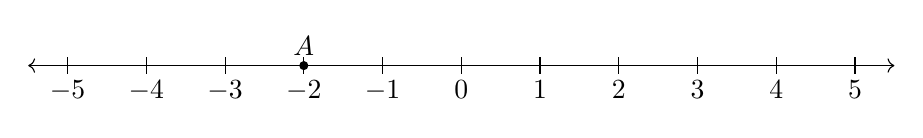
\begin{tikzpicture}
  \draw [<->] (-5.5,0)--(5.5,0);
  \foreach \x in {-5,...,5} %2 leading for diff!=1
    \draw[shift={(\x,0)},color=black] (0pt,-3pt) -- (0pt,3pt) node[below=5pt]  {$\x$};
    \draw [fill] (-2,0) circle [radius=0.05] node[above] {$A$};
\end{tikzpicture}

\begin{center} %4 quadrant regents grid
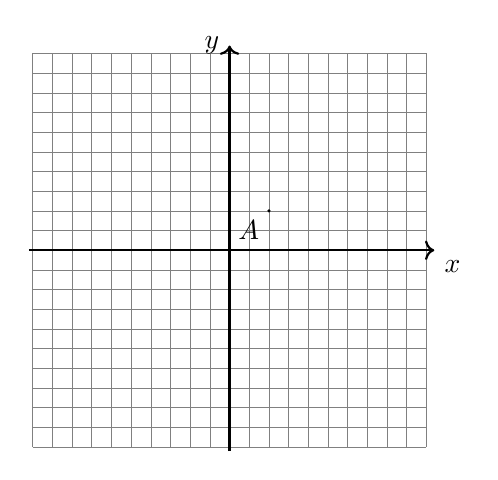
\begin{tikzpicture}[scale=.25]%[scale=0.635]
  \draw [help lines] (-10,-10) grid (10,10);
  \draw [thick, ->] (-10.2,0) -- (10.4,0) node [below right] {$x$};
  \draw [thick, ->] (0,-10.2)--(0,10.4) node [left] {$y$};
  \draw[fill] (2,2) circle  [radius=0.05]
       node[below left] (4, 2) {$A$};
\end{tikzpicture}
\end{center}


\begin{center} %4 quadrant regents grid w T-chart
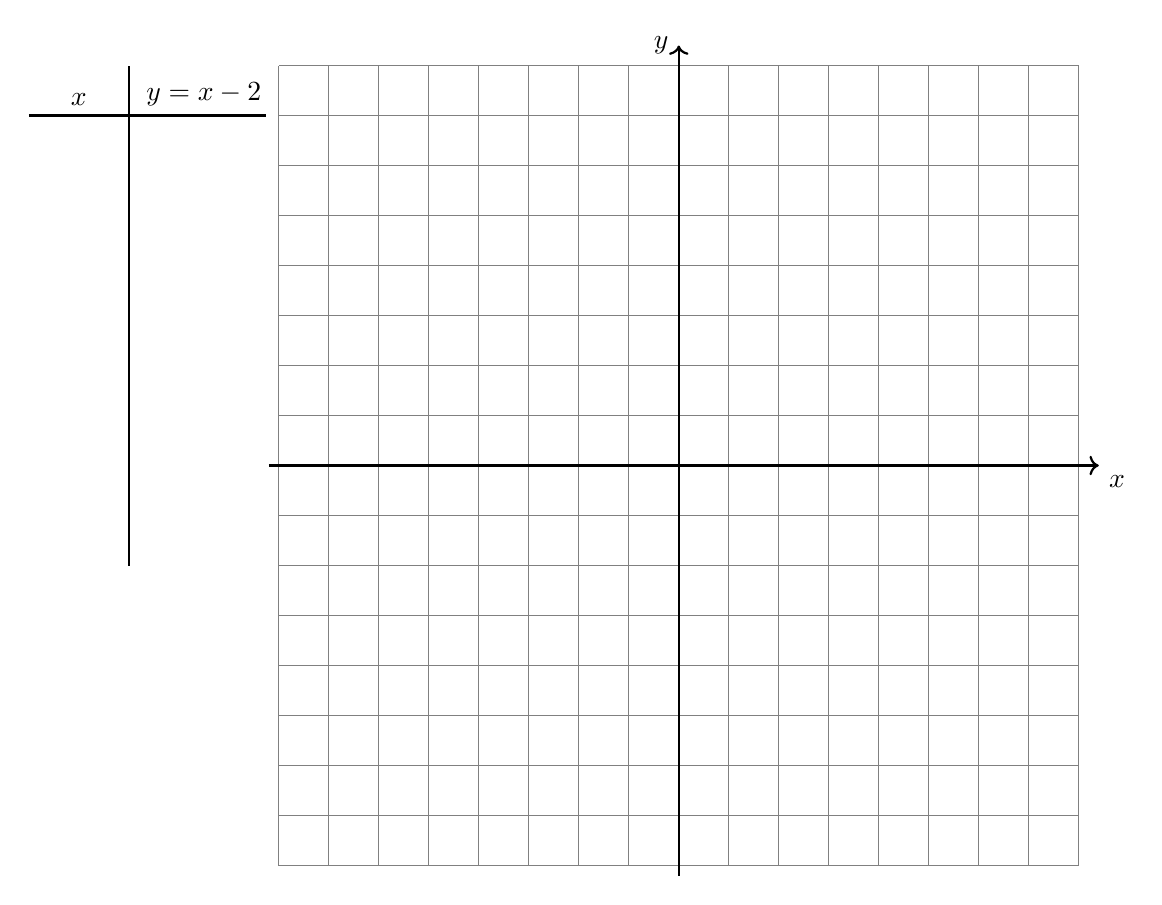
\begin{tikzpicture}[scale=.635]%[scale=0.635]
  \draw [thick, -] (-11, -2)--(-11,8);
  \draw [thick, -] (-13,7)--(-8.25,7);
  \node at (-12,7) [above] {$x$};
  \node at (-9.5,7) [above] {$y=x-2$};
  \draw [help lines] (-8,-8) grid (8,8);
  \draw [thick, ->] (-8.2,0) -- (8.4,0) node [below right] {$x$};
  \draw [thick, ->] (0,-8.2)--(0,8.4) node [left] {$y$};
\end{tikzpicture}
\end{center}

Triangle $DAN$ is graphed on the set of axes below. % Regents June 2018 #15
The vertices of $\triangle DAN$ have coordinates $D(-6,-1), A(6,3), \text{ and } N(-3,10)$.\\
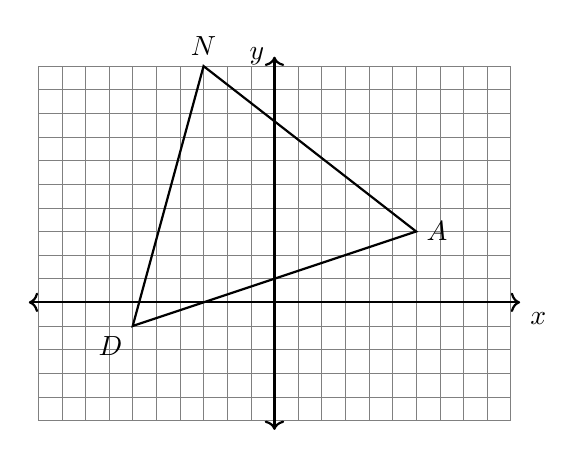
\begin{tikzpicture}[scale=.3]%[scale=0.635]
  \draw [help lines] (-10,-5) grid (10,10);
  \draw [thick, <->] (-10.4,0) -- (10.4,0) node [below right] {$x$};
  \draw [thick, <->] (0,-5.4)--(0,10.4) node [left] {$y$};
  \draw [-, thick] (-6,-1) node[below left]{$D$} --
    (6,3) node[right]{$A$} --(-3,10) node[above]{$N$} --cycle;
\end{tikzpicture}\\
What is the area of $\triangle DAN$?

\begin{tikzpicture}[->] %3 dimensions
  \draw (0,0) -- (1,0);
  \draw (0,0) -- (0,1,0);
  \draw (0,0) -- (0,0,1);
\end{tikzpicture}

\begin{figure} %[!htbp] First quadrant with axes
  \caption{$x$ and $y$ axes for grid}
  \centering
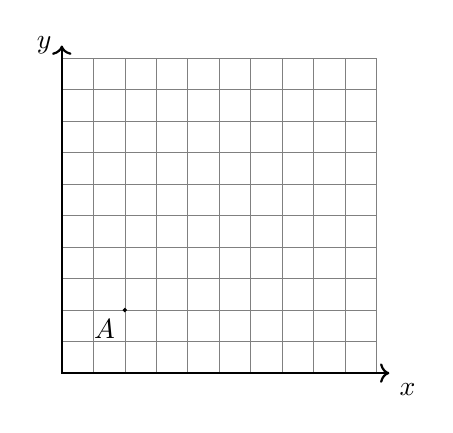
\begin{tikzpicture}[scale=0.4]
  \draw [help lines] (0,0) grid (10,10);
  \draw [thick, <->] (0,10.4) node [left] {$y$}
       -- (0,0) -- (10.4,0) node [below right] {$x$};
  \draw[fill] (2,2) circle  [radius=0.05]
       node[below left] (2, 2) {$A$};
\end{tikzpicture}
\end{figure}

\subsubsection*{plot functions}
Use brackets around expressions, especially those having parenthesis\\
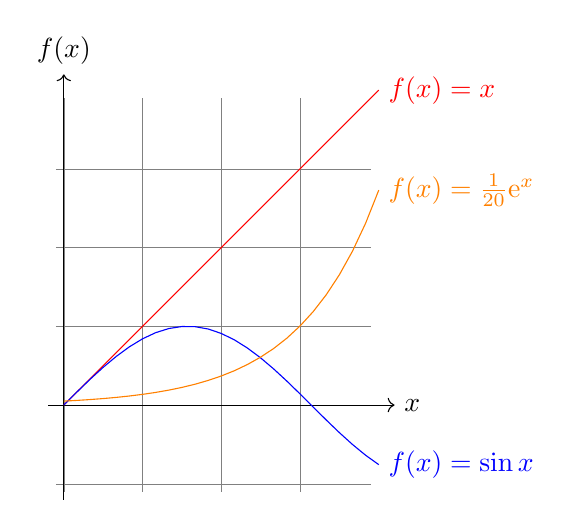
\begin{tikzpicture}[domain=0:4]
  \draw[very thin,color=gray] (-0.1,-1.1) grid (3.9,3.9);
  \draw[->] (-0.2,0) -- (4.2,0) node[right] {$x$};
  \draw[->] (0,-1.2) -- (0,4.2) node[above] {$f(x)$};
  \draw[color=red] plot (\x,\x) node[right] {$f(x) =x$};
  % \x r means to convert ’\x’ from degrees to _r_adians:
  \draw[color=blue] plot (\x,{sin(\x r)}) node[right] {$f(x) = \sin x$}; \draw[color=orange] plot (\x,{0.05*exp(\x)}) node[right] {$f(x) = \frac{1}{20} \mathrm e^x$};
\end{tikzpicture}

Axis numbering\\
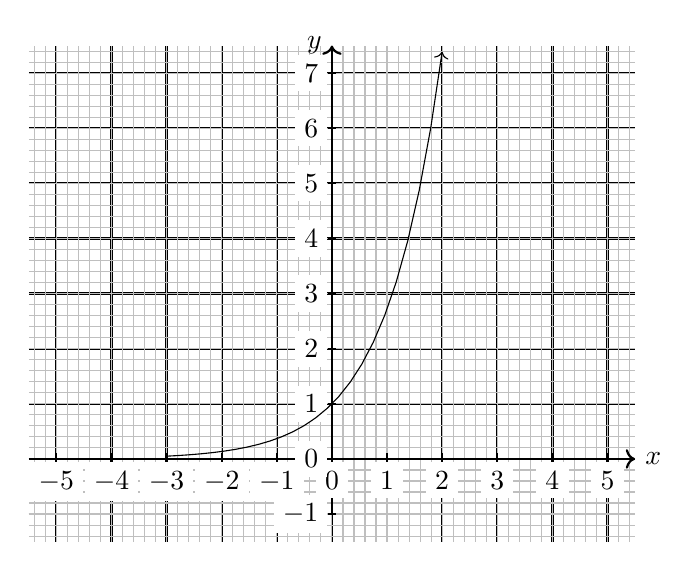
\begin{tikzpicture}[scale=0.7] %grid with numbered axes, IB cm paper.
  \draw [thick, color=black,, xstep=1.0cm,ystep=1.0cm] (-5.5,-1.5) grid (5.5,7.5);
  \draw [thin, color=lightgray,, xstep=0.2cm,ystep=0.2cm] (-5.5,-1.5) grid (5.5,7.5);
  \draw [thick, ->] (-5.5,0) -- (+5.5,0) node [right] {$x$};
  \draw [thick, ->] (0,-1.0) -- (0,7.5) node [left] {$y$};
  \foreach \x in {-5, -4, -3, -2, -1, 0,1,2,3,4,5}
    \draw[shift={(\x,0)},color=black] (0pt,-3pt) -- (0pt,3pt) node[below=3pt, fill=white]  {$\x$};
  \foreach \y in {-1,0,1,2,3,4,5, 6, 7}
    \draw[shift={(0,\y)},color=black] (2pt,0pt) -- (-2pt,0pt) node[left, fill=white]  {$\y$};

  \draw [<-, ->] plot[domain= -3:2] (\x, e^\x);
\end{tikzpicture}

\newpage

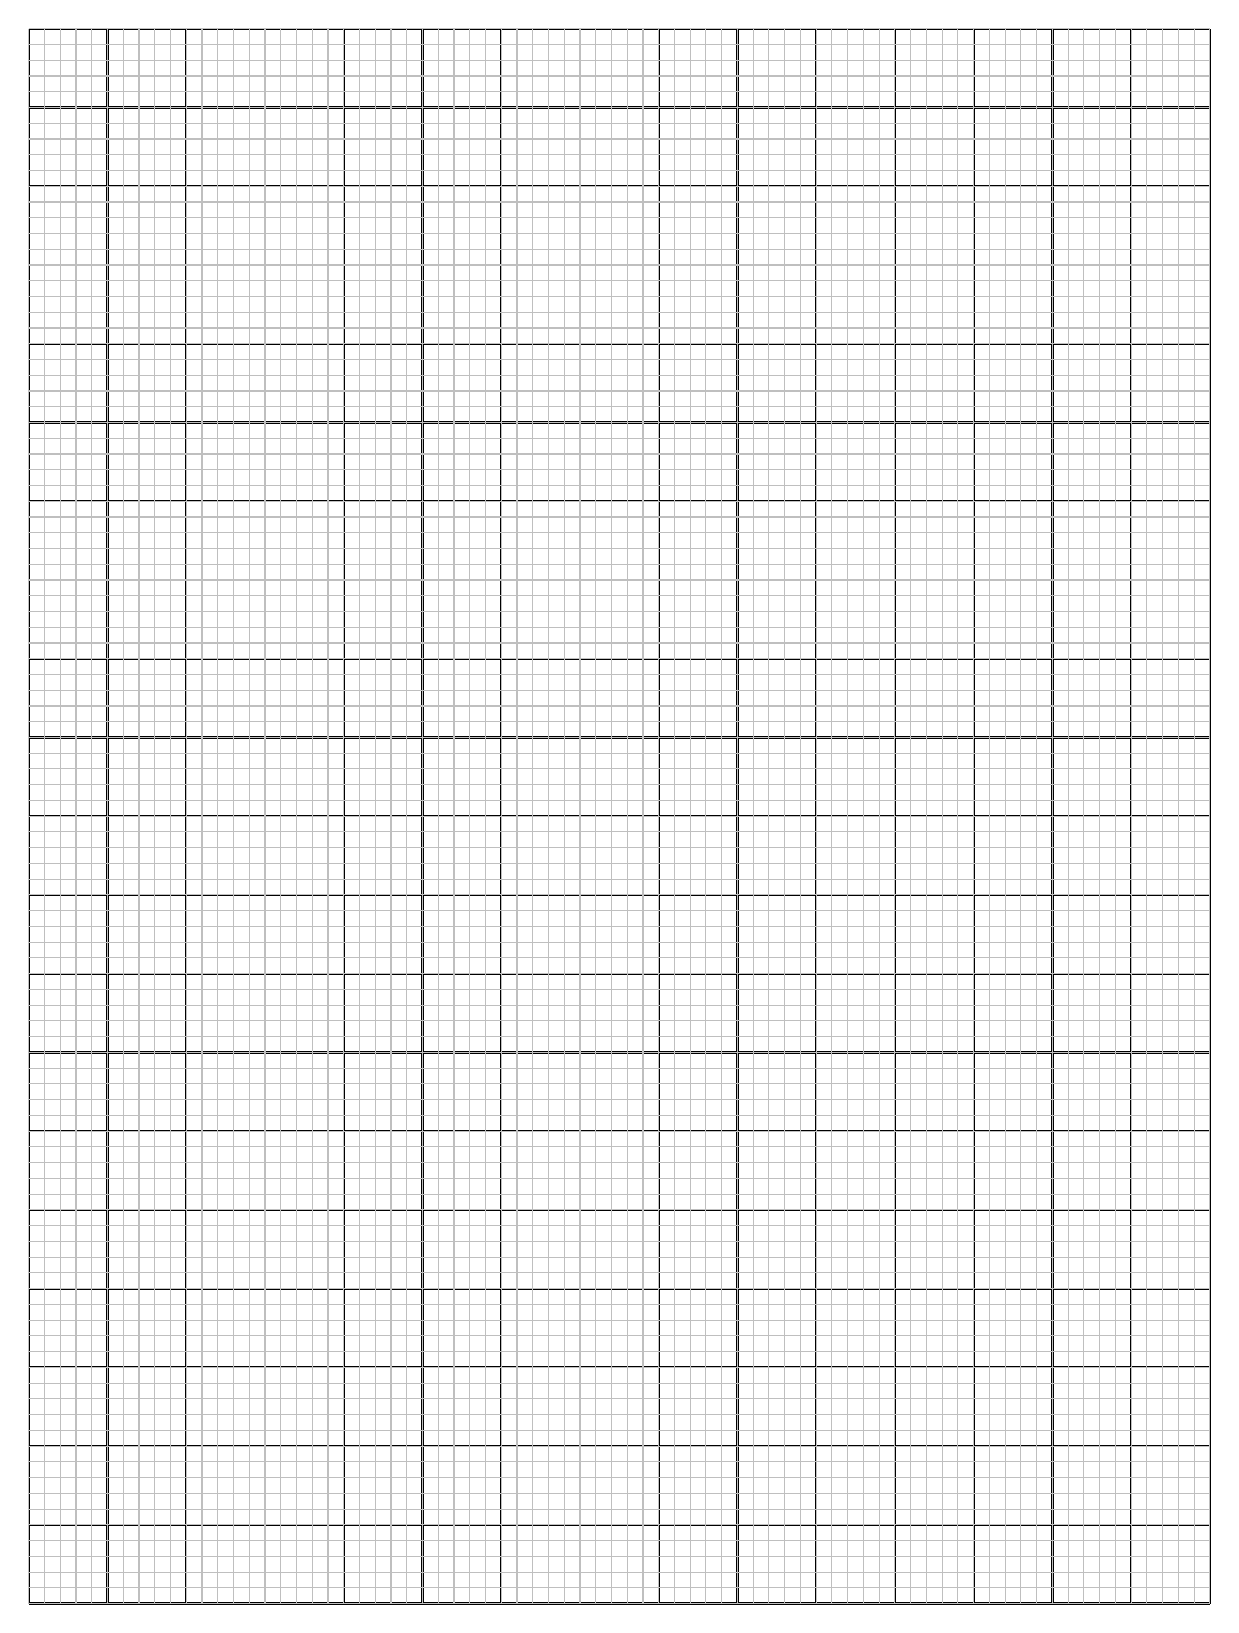
\begin{tikzpicture}[scale=1] %grid full page without axes, IB cm paper.
  \draw [thick, color=black,, xstep=1.0cm,ystep=1.0cm] (0,0) grid (15,20);
  \draw [thin, color=lightgray,, xstep=0.2cm,ystep=0.2cm] (0,0) grid (15,20);
  %\foreach \x in {-5, -4, -3, -2, -1, 0,1,2,3,4,5}
    %\draw[shift={(\x,0)},color=black] (0pt,-3pt) -- (0pt,3pt) node[below]  {$\x$};
  %\foreach \y in {-1,0,1,2,3,4,5, 6, 7}
    %\draw[shift={(0,\y)},color=black] (2pt,0pt) -- (-2pt,0pt) node[left]  {$\y$};
  %\draw [thick, ->] (-5.5,0) -- (+5.5,0) node [right] {$x$};
  %\draw [thick, ->] (0,-1.0) -- (0,7.5) node [left] {$y$};

  %\draw [<-, ->] plot[domain= -3:2] (\x, e^\x);
\end{tikzpicture}

\newpage


\subsubsection*{Drawing lines and shapes}
tikz draw command, node labeling function\\
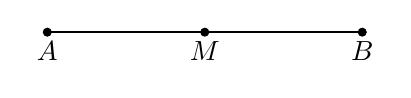
\begin{tikzpicture}
  \draw [-, thick] (1,0)--(5,0);
  \draw [fill] (1,0) circle [radius=0.05] node[below]{$A$};
  \draw [fill] (5,0) circle [radius=0.05] node[below]{$B$};
  \draw [fill] (3,0) circle [radius=0.05] node[below]{$M$};
\end{tikzpicture}

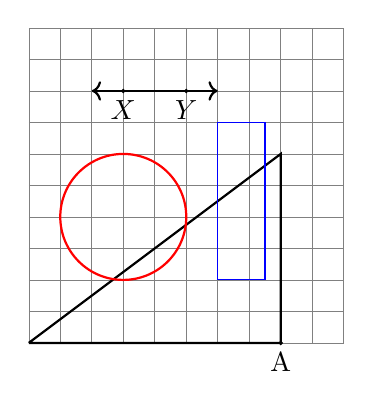
\begin{tikzpicture}[scale=0.4]
  \draw [help lines] (0,0) grid (10,10);
  \draw [thick](0,0)--(8,0)--(8,6)--(0,0); %Triangle
  \draw [fill] (8,0) circle [radius=0.05];
  \node [below] at (8,0) {A}; %above, right, left
  %line through points
  \draw [<->, thick] (2,8)--(6,8); % also thin, ultra thick, help lines, dashed, dotted, red
  \draw [fill] (3,8) circle [radius=0.05] node[below]{$X$};
  \draw [fill] (5,8) circle [radius=0.05] node[below]{$Y$};
  %shapes
  \draw [blue] (6,2) rectangle (7.5,7);
  \draw [red, thick] (3,4) circle [radius=2];
\end{tikzpicture}

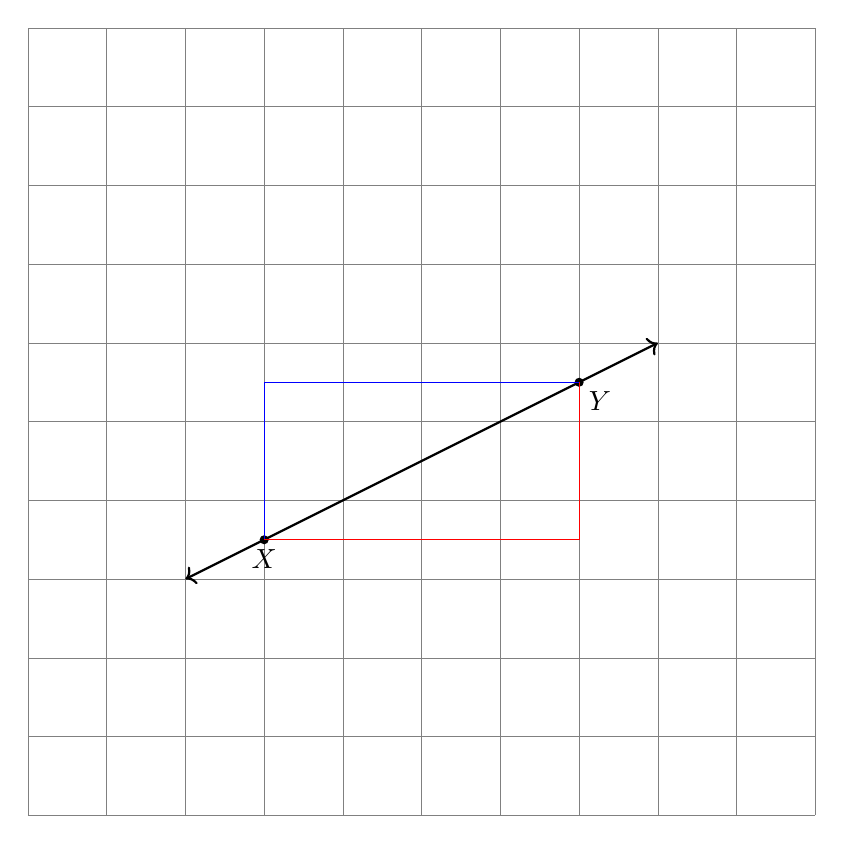
\begin{tikzpicture}%[scale=0.4]
  \draw [help lines] (0,0) grid (10,10);
  \draw [<->, thick] (2,3)--(8,6);
  \draw [fill] (3,3.5) circle [radius=0.05] node[below]{$X$};
  \draw [fill] (7,5.5) circle [radius=0.05] node[below right]{$Y$};
  \draw [color=blue] (3,3.5)--(3,3.5 |- 7,5.5)--(7,5.5);
  \draw [color=red] (3,3.5)--(7,5.5 |- 3,3.5)--(7,5.5);
\end{tikzpicture}

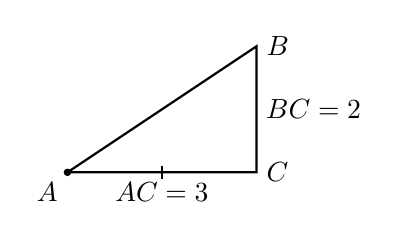
\begin{tikzpicture}[scale=0.8]
  \draw[fill] (2,2) circle  [radius=0.05]
       node[below left] (2, 2) {$A$};
  \draw [thick] (2,2)-- node[below]{$AC=3$} (5,2) node[right] {$C$} --(5,4) node[right] {$B$} --(2,2);
  \draw [thick] (3.5,2.1)--(3.5,1.9); %tick mark
  \node [right] at (5,3) {$BC=2$};
\end{tikzpicture}\vspace{1cm}

Given $\triangle ABC$ with $\overline{AC} \cong \overline{BC}$. $AC=x+7$ and $BC=2x+1$. Find $AC$.\\[0.5cm]
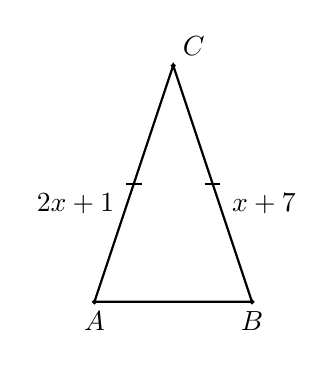
\begin{tikzpicture}[scale=0.5]
  \draw [thick](0,0)--(4,0)--(2,6)--(0,0);
  \draw [fill] (0,0) circle [radius=0.05] node[below]{$A$};
  \draw [fill] (4,0) circle [radius=0.05] node[below]{$B$};
  \draw [fill] (2,6) circle [radius=0.05] node[above right]{$C$};
  \draw [thick] (0.8,3)--(1.2,3); %tick mark
  \draw [thick] (2.8,3)--(3.2,3); %tick mark
  \node [right] at (3.25,2.5){$x+7$};
  \node [left] at (0.75,2.5){$2x+1$};
\end{tikzpicture}

\begin{center}
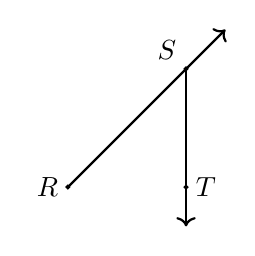
\begin{tikzpicture}[scale=0.5]
  \draw [->, thick] (0,0)--(4,4);
  \draw [->, thick] (3,3)--(3,-1);
  \draw [fill] (0,0) circle [radius=0.05] node[left]{$R$};
  \draw [fill] (3,3) circle [radius=0.05] node[above left]{$S$};
  \draw [fill] (3,0) circle [radius=0.05] node[right]{$T$};
\end{tikzpicture}
\end{center}

\subsubsection*{Triangles}

Shift using coordinates\\
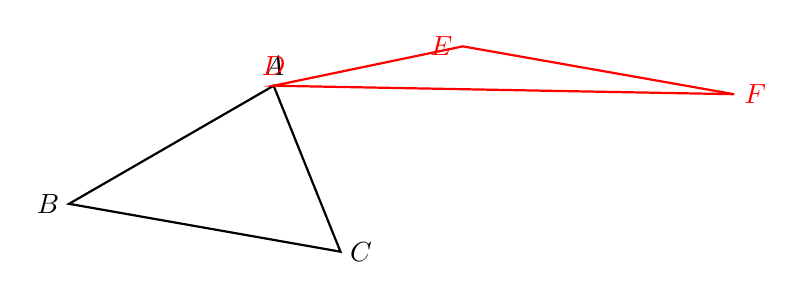
\begin{tikzpicture}
  \coordinate [label=above:$A$](A) at (30:3);
  \coordinate [label=left:$B$](B) at (0, 0);
  \coordinate [label=right:$C$](C) at (-10:3.5);
  \draw [thick] (A)--(B)--(C)--cycle;

  \draw [thick, red, xshift=5cm, yshift=2cm] (A) node[above]{$D$}--
  (0,0) node[left]{$E$}--
  (-10:3.5) node[right]{$F$}--cycle;
\end{tikzpicture}

Shift and rotate\\
\begin{tikzpicture}
  \coordinate [label=above:$A$](A) at (30:3);
  \coordinate [label=left:$B$](B) at (0, 0);
  \coordinate [label=right:$C$](C) at (-10:3.5);
  \draw [thick] (A)--(B)--(C)--cycle;

  \draw [thick, red, xshift=5cm, yshift=2cm, rotate=45] (30:3) node[above]{$D$}--
  (0,0) node[left]{$E$}--
  (-10:3.5) node[right]{$F$}--cycle;
\end{tikzpicture}

Scale\\
\begin{tikzpicture}
  \coordinate [label=above:$A$](A) at (30:3);
  \coordinate [label=left:$B$](B) at (0, 0);
  \coordinate [label=right:$C$](C) at (-10:3.5);
  \draw [thick] (A)--(B)--(C)--cycle;

  \draw [dashed, red, scale=2] (30:3) node[above]{$D$}--
  (0,0) node[left]{$E$}--
  (-10:3.5) node[right]{$F$}--cycle;
\end{tikzpicture}

Reflect\\
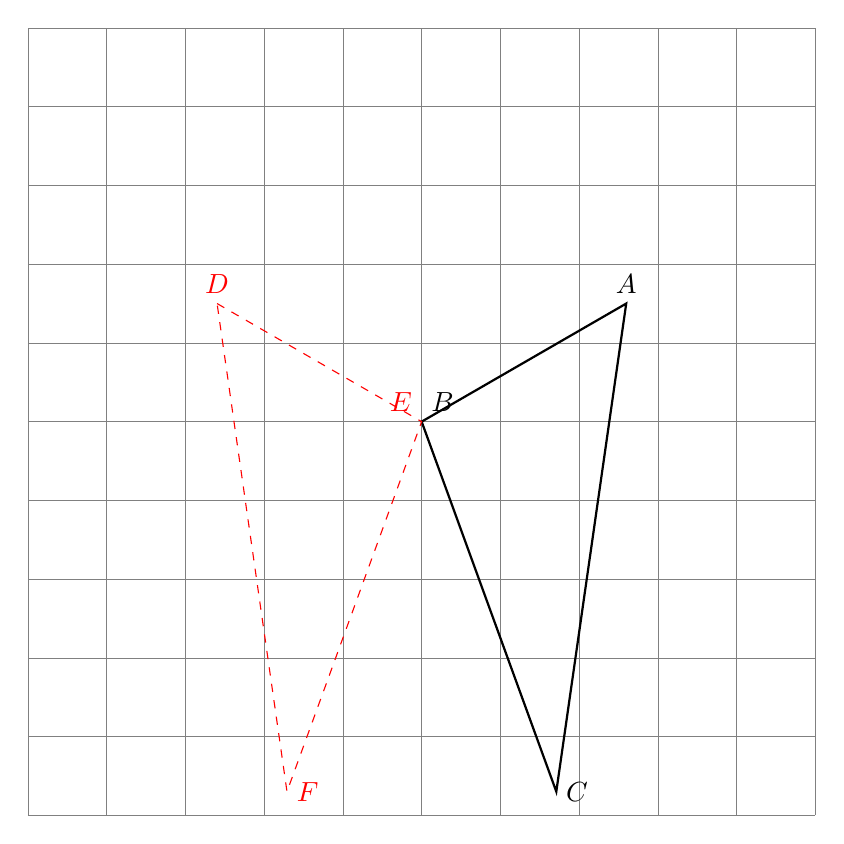
\begin{tikzpicture}
  \draw [help lines] (-5,-5) grid (5,5);
  \coordinate [label=above:$A$](A) at (30:3);
  \coordinate [label=above right:$B$](B) at (0, 0);
  \coordinate [label=right:$C$](C) at (-70:5);
  \draw [thick] (A)--(B)--(C)--cycle;
  \draw [dashed, red, xscale=-1] (30:3) node[above]{$D$}--
  (0,0) node[above left]{$E$}--
  (-70:5) node[right]{$F$}--cycle;
\end{tikzpicture}

\subsubsection*{Complex Regents angle problems}

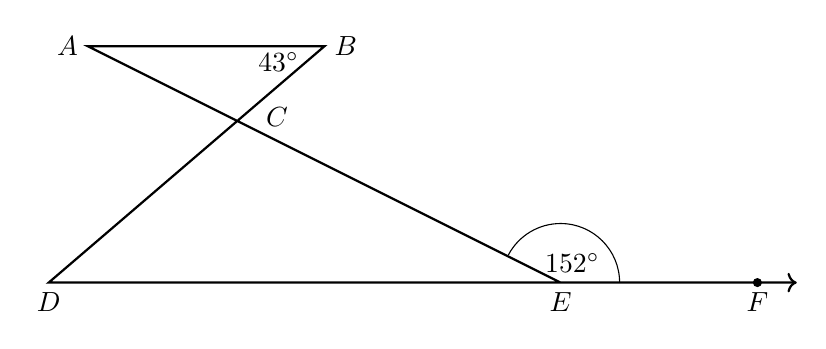
\begin{tikzpicture}%[scale=0.5] %Regents June 2018 #2
  \draw [->, thick] (6.5,0) node[below]{$E$} --
    (0.5,3) node[left]{$A$} --(3.5,3) node[right]{$B$} --
    (0,0) node[below]{$D$} -- (9,0) node[below]{$F$} -- (9.5,0);
  \draw [fill] (9,0) circle [radius=0.05];
  \node at (2.9,2.1)[ ]{$C$};
  \node at (6.65,0)[above]{$152^\circ$};
  \node at (3.3,3.05)[below left]{$43^\circ$};
  \draw (6.5,0) +(0.75,0) arc [start angle=0, end angle=152, radius=0.75];
\end{tikzpicture}

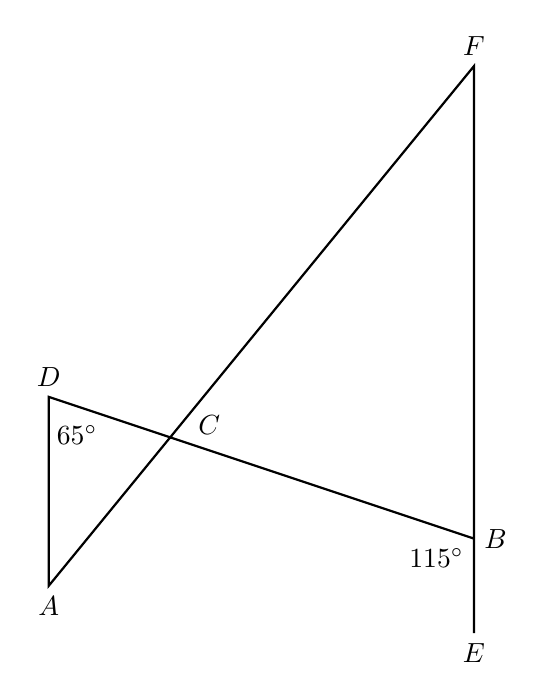
\begin{tikzpicture}[scale=1.2] %Regents June 2018 #4
  \draw [-, thick] (4.5,0.5) node[right]{$B$} --
    (4.5,5.5) node[above]{$F$} --(0,0) node[below]{$A$} --
    (0,2) node[above]{$D$} -- (4.5,0.5) node[below left]{$115^\circ$} -- (4.5,-0.5)node[below]{$E$};
  %\draw [fill] (9,0) circle [radius=0.05];
  \node at (1.7,1.7)[ ]{$C$};
  \node at (0.3,1.6)[ ]{$65^\circ$};
  %\node at (3.3,3.05)[below left]{$43^\circ$};
  %\draw (6.5,0) +(0.75,0) arc [start angle=0, end angle=152, radius=0.75];
\end{tikzpicture}


Given the rectangle $ABCD$ with $\overline{AB} \cong \overline{CD}$ and $\overline{BC} \cong \overline{DA}$. $AB=x+7$ and $\displaystyle CD=\frac{4x+2}{2}$. Find $AB$.\\[0.5cm]
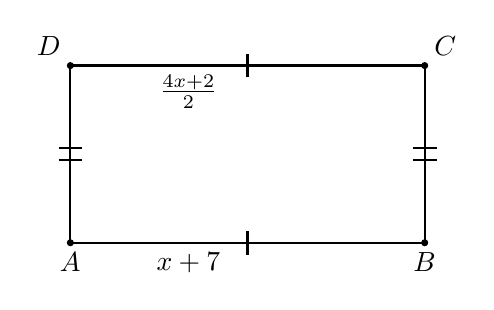
\begin{tikzpicture}[scale=0.75]
  \draw [thick](0,0)--(6,0)--(6,3)--(0,3)--cycle;
  \draw [fill] (0,0) circle [radius=0.05] node[below]{$A$};
  \draw [fill] (6,0) circle [radius=0.05] node[below]{$B$};
  \draw [fill] (6,3) circle [radius=0.05] node[above right]{$C$};
  \draw [fill] (0,3) circle [radius=0.05] node[above left]{$D$};
  \draw [thick] (3,-0.2)--(3,0.2); %tick mark
  \draw [thick] (3,2.8)--(3,3.2); %tick mark
  \draw [thick] (-0.2,1.4)--(0.2,1.4); %tick mark
  \draw [thick] (-0.2,1.6)--(0.2,1.6); %tick mark
  \draw [thick] (5.8,1.4)--(6.2,1.4); %tick mark
  \draw [thick] (5.8,1.6)--(6.2,1.6); %tick mark
  \node [below] at (2,0){$x+7$};
  \node [below] at (2,3){$\frac{4x+2}{2}$};
\end{tikzpicture}

\subsection*{Plane geometry}
  Identify two lines in the given plane.\\
  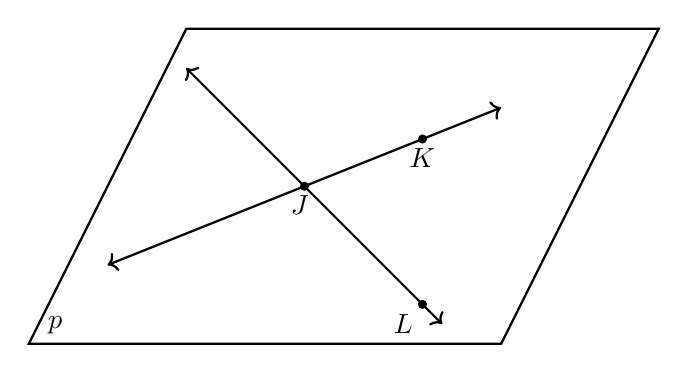
\begin{tikzpicture}
    \draw [thick](0,0) node[above right]{$\ p$} --(6,0)--(8,4)--(2,4)--cycle;
    \draw [<->, thick] (1,1)--(6,3);
    \draw [fill] (3.5,2) circle [radius=0.05] node[below]{$J \ $};
    \draw [fill] (5,2.6) circle [radius=0.05] node[below]{$K$};
    \draw [<->, thick] (2,3.5)--(5.25,.25);
    \draw [fill] (5,0.5) circle [radius=0.05] node[below left]{$L$};
  \end{tikzpicture} \vspace{2cm}

\subsection*{Marking angles}
\begin{tikzpicture} %[scale=3]
  \draw [<->, thick] (37:5) node[above]{$A$} --(0,0)node[label=left:$B$]{} --(5,0);
  \draw [color=blue] (0.75,0) arc [start angle=0, end angle=37, radius=0.75];
\end{tikzpicture}\vspace{0.5cm}

\begin{tikzpicture}
\draw (3,0) coordinate (A)
         -- (0,1) coordinate (B)
         -- (1,2) coordinate (C)
            pic [draw, "$\alpha$"] {angle};
\end{tikzpicture}

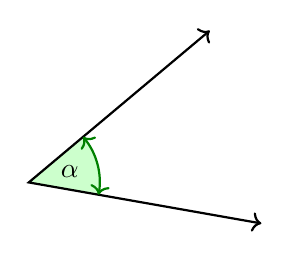
\begin{tikzpicture}
  \coordinate (A) at (40:3);
  \coordinate (B) at (0, 0);
  \coordinate (C) at (-10:3);
  \draw [<->, thick] (A)--(B)--(C)
  %pic [draw=black, angle radius=0.4, "$\theta$"]{angle = A--B--C};
  pic [draw=green!50!black, fill=green!20, angle radius=9mm,
             "$\alpha$"] {angle = C--B--A};
\end{tikzpicture}

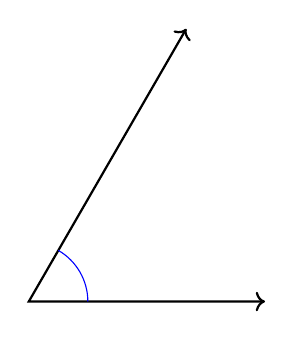
\begin{tikzpicture} %[scale=3]
  \draw [<->, thick] (3,0)--(0,0)--(60:4); %note polar coordinates
  \draw [color=blue] (0.75,0) arc [start angle=0, end angle=60, radius=0.75];
\end{tikzpicture}\vspace{1cm}

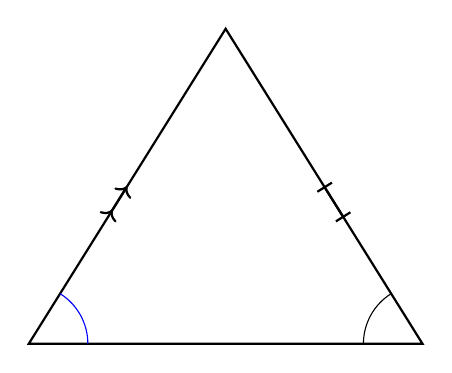
\begin{tikzpicture} %[scale=3] Isosceles, parallel marks, congruence marks
  \draw [-, thick] (0,0)--(5,0)--(2.5,4)--cycle;
  \draw [>->, thick] (1.0,1.6)--(1.25,2);
  \draw [{Bar[]}-{Bar[]}, thick] (4,1.6)--(3.75,2);
  \draw [color=blue] (0.75,0) arc [start angle=0, end angle=58, radius=0.75];
  \draw (5,0)-- +(-0.75,0) arc [start angle=180, end angle=122, radius=0.75];
\end{tikzpicture}\vspace{1cm}

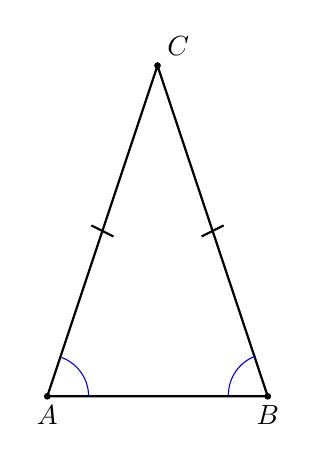
\begin{tikzpicture}[scale=0.7]
  \draw [thick](0,0)--(4,0)--(2,6)--(0,0);
  \draw [fill] (0,0) circle [radius=0.05] node[below]{$A$};
  \draw [fill] (4,0) circle [radius=0.05] node[below]{$B$};
  \draw [fill] (2,6) circle [radius=0.05] node[above right]{$C$};
  \draw [color=blue] (0,0) ++(0.75,0) arc [start angle=0, end angle=70, radius=0.75];
  \draw [color=blue] (4,0) ++(-0.22, 0.73) arc [start angle=110, end angle=180, radius=0.75];
  \draw [thick] (0.8,3.1)--(1.2,2.9); %tick mark
  \draw [thick] (2.8,2.9)--(3.2,3.1); %tick mark
  %\node [right] at (3.25,2.5){$x+7$};
  %\node [left] at (0.75,2.5){$2x+1$};
\end{tikzpicture}

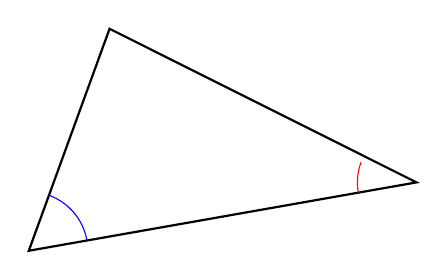
\begin{tikzpicture} %[scale=3]
  \draw [-, thick] (10:5)--(0,0)--(70:3)--cycle;
  \draw [color=blue] (0,0) ++(10:0.75) arc [start angle=10, end angle=70, radius=0.75];
  \draw [color=red] (10:5) ++(190:0.75) arc [start angle=190, end angle=160, radius=0.75];
\end{tikzpicture}\vspace{1cm}

\tikz \draw (2,0) coordinate (A) -- (0,0) coordinate (B)
         -- (1,1) coordinate (C)
  pic ["$K$", draw, ->] {angle=A--B--C};

  \begin{tikzpicture}
    \draw
      (3,-1) coordinate (a) node[right] {a}
      -- (0,0) coordinate (b) node[left] {b}
      -- (2,2) coordinate (c) node[above right] {c}
      pic["$\alpha$", draw=orange, <->, angle eccentricity=1.2, angle radius=1cm]
      {angle=a--b--c};
  \end{tikzpicture}

\subsection*{Circles}
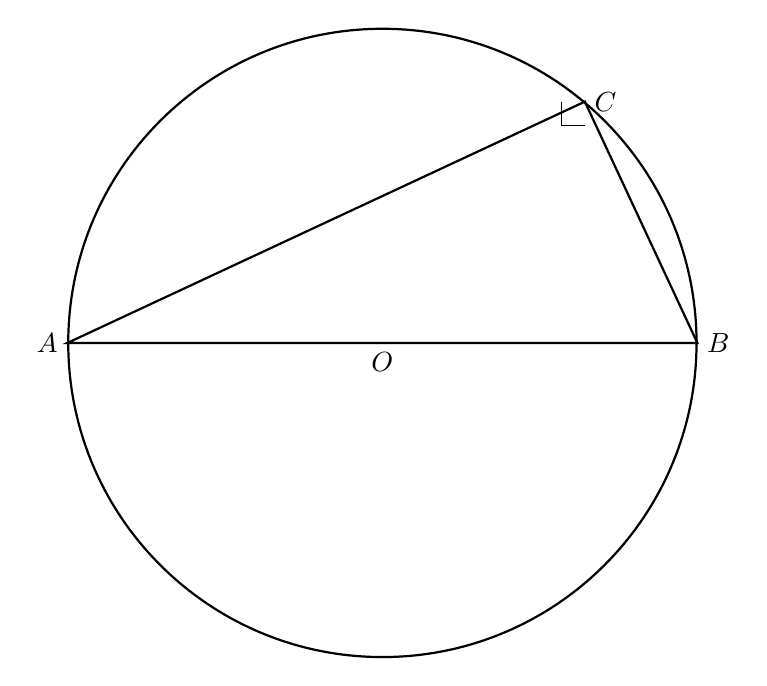
\begin{tikzpicture}
  \coordinate [label=left:$A$] (A) at (-4,0);
  \coordinate [label=right:$B$] (B) at (4,0);
  \coordinate [label=right:$C$] (C) at (50:4);
  \node [draw,circle through=(C), thick] at (0,0){};
  \node at (0,0)[below]{$O$};
  \draw[thick] (A) -- (B)--(C)--cycle;
  \draw (C) ++(-0.3,0)-- +(0,-0.3)-- +(0.3,-0.3);
\end{tikzpicture}

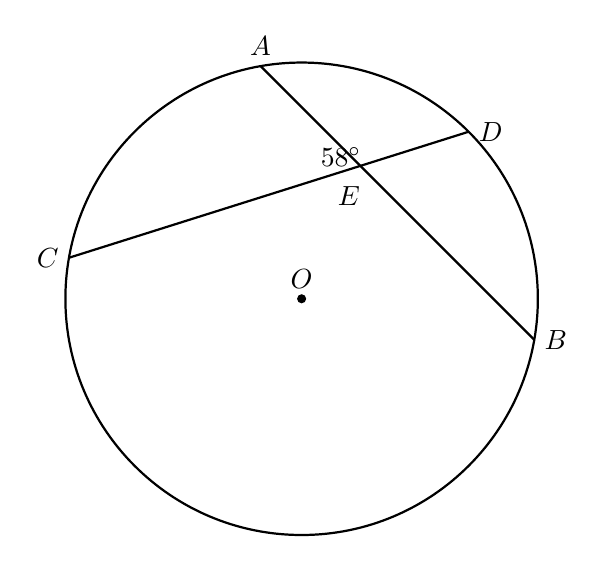
\begin{tikzpicture}
  \draw [thick] (0,0) circle [radius=3cm] node[above]{$O$};
  \draw [fill] (0,0) circle [radius=0.5mm];
  \draw [-,thick] (170:3) node[left]{$C$} -- (45:3) node[right]{$D$};
  \draw [-,thick] (100:3) node[above]{$A$} --  (-10:3) node[right]{$B$};
  \node at (0.5,1.8) {$58^\circ$};
  \node at (0.6,1.3) {$E$};
\end{tikzpicture}

\end{document}
